\documentclass[12pt,a4paper]{article}

\usepackage[utf8]{inputenc}
\usepackage[T1]{fontenc}
\usepackage[czech]{babel}
\usepackage{lmodern}
\usepackage{graphicx}
\usepackage{float}
\usepackage{hyperref}
\usepackage{geometry}
\usepackage{xcolor}
\usepackage{tcolorbox}
\usepackage{parskip}
\usepackage{booktabs}
\usepackage{tabularx}
\usepackage{listings}
\usepackage{amsmath}
\usepackage[nopatch=item]{microtype}
\usepackage{xurl}
\usepackage{etoolbox}
\usepackage{fancyhdr}
\usepackage{titlesec}
\usepackage[font=small,labelfont={bf,color=primaryblue},labelsep=space]{caption}

% Allow line breaking and hyphenation in typewriter font (\texttt) without font warnings
\apptocmd{\ttfamily}{\hyphenchar\font=45}{}{}

\geometry{margin=2.5cm, headheight=15pt}

% Color definitions (matching CSGDB design palette)
\definecolor{primaryblue}{RGB}{25, 118, 210}
\definecolor{darkblue}{RGB}{13, 71, 161}
\definecolor{lightbg}{RGB}{245, 247, 250}
\definecolor{accentblue}{RGB}{227, 242, 253}

\hypersetup{
    colorlinks=true,
    linkcolor=primaryblue,
    urlcolor=primaryblue,
    pdftitle={Czech Salivary Gland Database --- Technologická dokumentace},
    pdfauthor={Západočeská univerzita v Plzni}
}

% Section styling
\titleformat{\section}
  {\Large\bfseries\color{darkblue}}
  {\thesection}{1em}{}[\color{primaryblue}\titlerule]

\titleformat{\subsection}
  {\large\bfseries\color{primaryblue}}
  {\thesubsection}{1em}{}

\titleformat{\subsubsection}
  {\normalfont\bfseries\color{darkblue}}
  {\thesubsubsection}{1em}{}

\usepackage[fit]{truncate}

% Header and Footer setup
\pagestyle{fancy}
\fancyhf{}
\fancyhead[L]{\small\color{gray}\textbf{CSGDB} --- Technologická dokumentace}
\fancyhead[R]{\small\color{gray}\truncate{0.45\textwidth}{\nouppercase{\leftmark}}}
\fancyfoot[L]{\small\color{gray}Západočeská univerzita v Plzni}
\fancyfoot[R]{\small\color{gray}\thepage}
\renewcommand{\headrulewidth}{0.4pt}
\renewcommand{\footrulewidth}{0.4pt}

% tcolorbox default style
\tcbset{
    colback=lightbg,
    colframe=primaryblue,
    fonttitle=\bfseries\color{white},
    coltitle=white,
    boxrule=0.8pt,
    arc=3pt
}

% Adjust spacing tolerance to eliminate overfull hboxes
\emergencystretch=3em

\begin{document}

% Custom Title Page
\begin{titlepage}
    \pagenumbering{alph}
    \pagecolor{white}
    \fontfamily{lmss}\selectfont
    \centering
    
    \vspace*{1.5cm}
    
    % Banner Logo
    
\includegraphics[width=0.85\textwidth]{img/LOGO_splt.png}
    
    \vspace{2cm}
    
    {\Huge \bfseries \color{darkblue} TECHNOLOGICKÁ DOKUMENTACE} \\[0.8em]
    {\Large \color{gray} Architektura a systémové moduly aplikace Czech Salivary Gland Database (CSGDB)}
    
    \vspace{1.5cm}
    
    \begin{tcolorbox}[colback=accentblue,colframe=primaryblue,arc=4pt,halign=center,width=0.6\textwidth]
        \centering \Large \bfseries \color{darkblue} Verze 3.0.9
    \end{tcolorbox}
    
    \vfill
    
    {\large \bfseries \color{darkblue} Západočeská univerzita v Plzni} \\[0.3em]
    {\small \color{gray} Fakulta aplikovaných věd --- Katedra informatiky a výpočetní techniky} \\[0.2em]
    {\small \color{gray} Ve spolupráci s Českou společností otorinolaryngologie a chirurgie hlavy a krku}
    
    \vspace{1cm}
    {\small \color{gray} Plzeň}
    
\end{titlepage}
\nopagecolor

\pagenumbering{arabic}
\pagestyle{fancy}
\tableofcontents
\newpage

\section{Architektura systému a komponenty}

Aplikace \textbf{CSGDB} je vícevrstvá desktopová platforma založená na rozhraní \textbf{Electron} (v29.x). Odděluje klientské uživatelské rozhraní (Renderer), aplikační a databázovou logiku (Main), meziprocesovou komunikaci (IPC) a externí modul pro strojové učení (Python ML Engine). Vizualizace kontejnerů architektury dle C4 modelu je znázorněna na Obrázku~\ref{fig:c4-level-2}.

\subsection{Přehled systémových vrstev}

\begin{table}[H]
\centering
\small
\begin{tabularx}{\textwidth}{l l X}
\toprule
\textbf{Vrstva / Modul} & \textbf{Adresář} & \textbf{Technologický stoh} \\
\midrule
Prezentační vrstva & \texttt{src/frontend} & React 18, TypeScript, MUI, Recharts, i18next \\
Aplikační backend & \texttt{src/backend} & Node.js, SQLite (\texttt{sqlite3}), AES-256-CBC \\
Meziprocesová komunikace & \texttt{src/ipc} & Electron IPC, \texttt{contextBridge}, DTOs \\
Strojové učení & \texttt{python-ml-engine} & Python 3.8+, \texttt{scikit-survival}, PyInstaller \\
\bottomrule
\end{tabularx}
\caption{Přehled vrstev a použitých technologií v CSGDB.}
\end{table}

\begin{tcolorbox}[title=Komponentový model systému]
\begin{itemize}
    \item \textbf{Frontend (\texttt{src/frontend}):} Vykreslování formulářů, správa seznamů pacientů, filtrace, statistické grafy Kaplan-Meier a predikce rizika.
    \item \textbf{Backend (\texttt{src/backend}):} Relace SQLite databáze, CRUD operace, šifrování PII údajů, exporty/importy a řízení běhu ML procesů.
    \item \textbf{IPC vrstva (\texttt{src/ipc}):} Asynchronní, typově bezpečné propojení rendereru a main procesu přes kanály a handlery.
    \item \textbf{Python ML Engine (\texttt{python-ml-engine}):} Binární služba pro trénování modelů přežití a výpočet skóre rizika přes \texttt{stdin}/\texttt{stdout} JSON rozhraní (vč. trvalého \textit{sidecar} režimu).
\end{itemize}
\end{tcolorbox}

\begin{figure}[H]
    \centering
    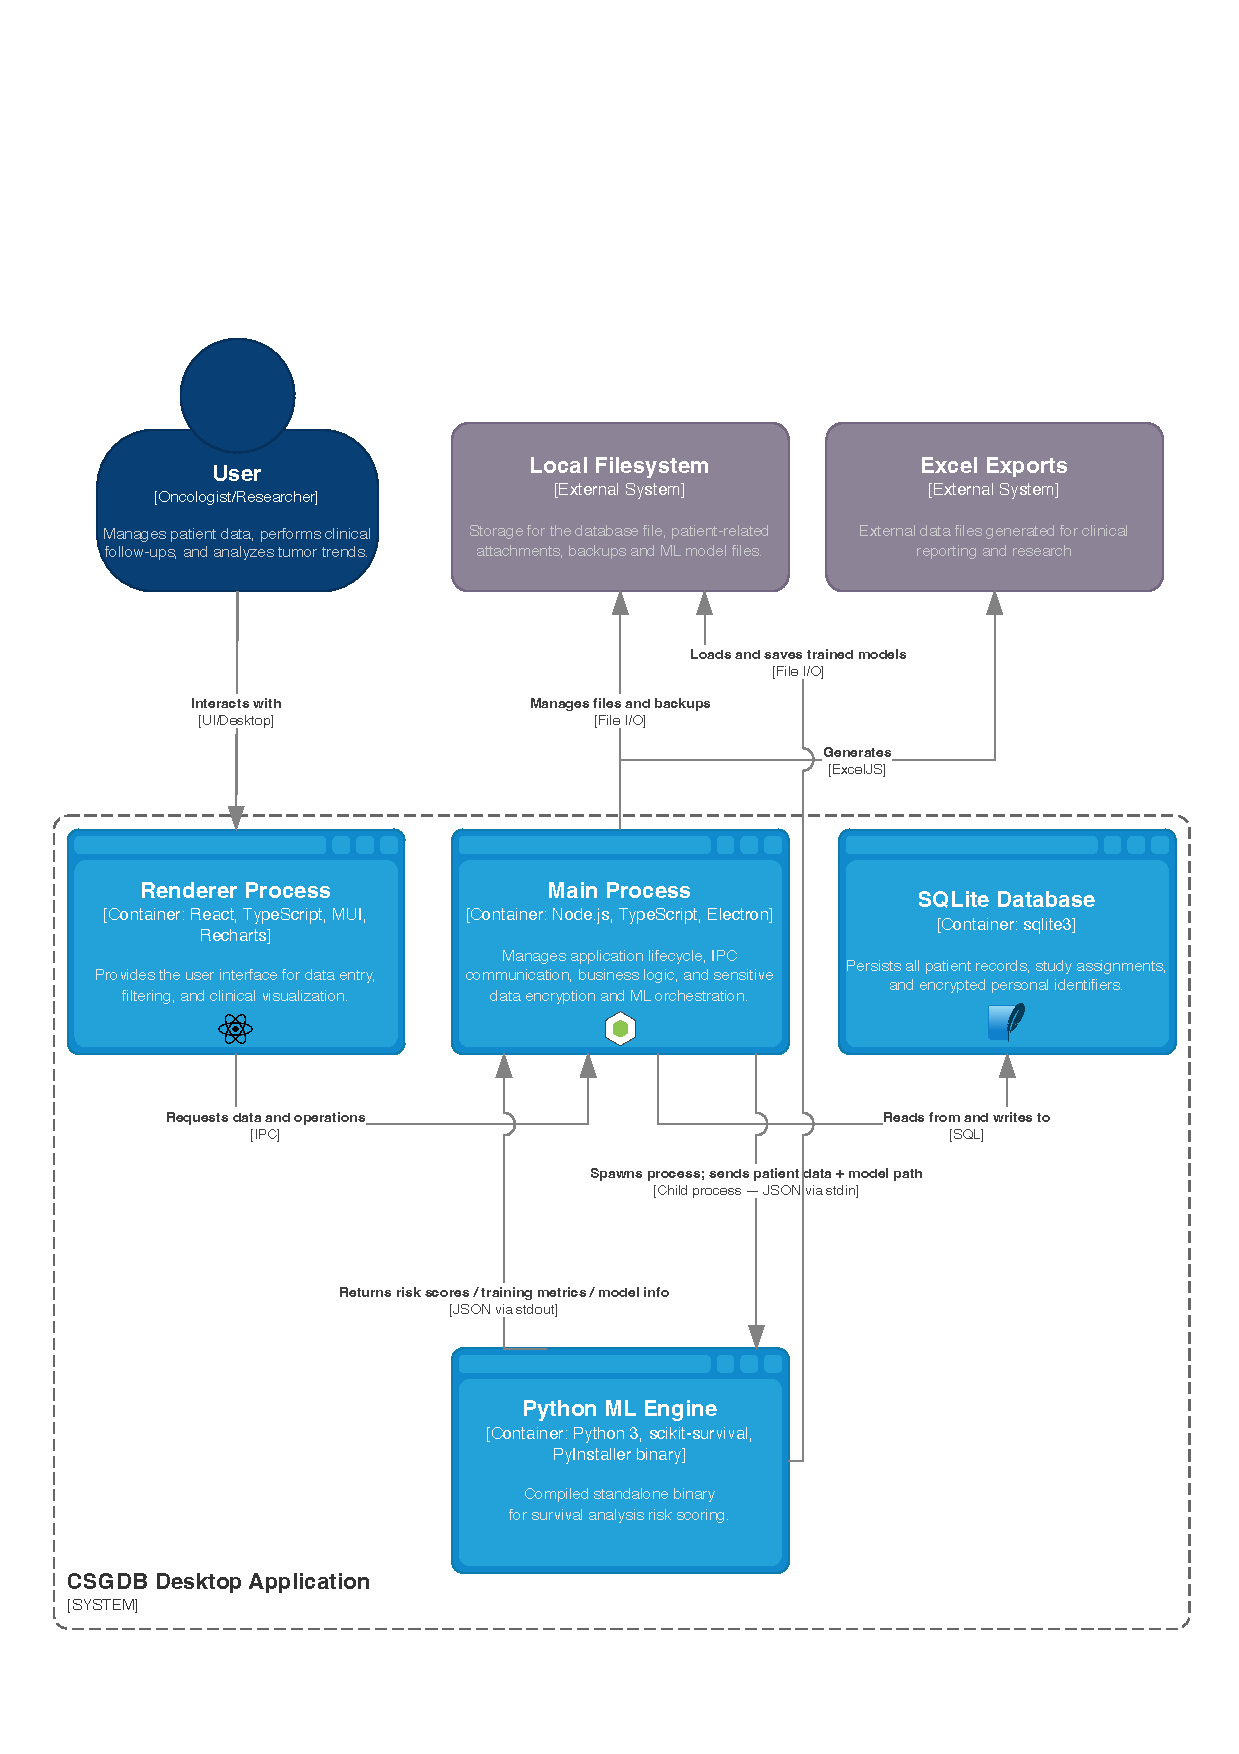
\includegraphics[width=0.95\textwidth]{img/C4-level-2-new.pdf}
    \caption{Diagram kontejnerů systému CSGDB (C4 model --- Level 2).}
    \label{fig:c4-level-2}
\end{figure}

---

\section{Prezentační vrstva --- Frontend (\texttt{src/frontend})}

Prezentační vrstva je vybudována v knihovně \textbf{React 18} za použití \textbf{TypeScriptu} a designového systému \textbf{Material UI (MUI)}.

\subsection{Struktura adresáře \texttt{src/frontend}}
\begin{itemize}
    \item \texttt{components/}: UI komponenty pro zobrazení pacientů, studií, filtraci a statistiky:
    \begin{itemize}
        \item Seznamy a detaily pacientů:
        \begin{itemize}
            \item \texttt{patients-list.tsx}
            \item \texttt{patient-button.tsx}
            \item \texttt{patient-risk-card.tsx}
        \end{itemize}
        \item Filtrační rozhraní:
        \begin{itemize}
            \item \texttt{filtration-malignant.tsx}
            \item \texttt{filtration-benign.tsx}
            \item \texttt{filtration-menu.tsx}
        \end{itemize}
        \item Správa studií: \texttt{studies-list.tsx}, \texttt{add-study.tsx}
        \item Vizualizace a statistika: \texttt{kaplan-meier.tsx}, \texttt{kaplan-meier-filter.tsx}, \texttt{statistics/}
        \item Sledování stavu ML: \texttt{ml-progress-widget.tsx}, \texttt{ml-operation-context.tsx}
    \end{itemize}
    \item \texttt{components/forms/}: Formulářové komponenty rozdělené podle typu slinné žlázy:
    \begin{itemize}
        \item Anatomičtí zástupci:
        \begin{itemize}
            \item Příušní žláza (\texttt{parotid/})
            \item Podčelistní žláza (\texttt{submandibular/})
            \item Podjazyková žláza (\texttt{sublingual/})
        \end{itemize}
        \item Formulářové sekce:
        \begin{itemize}
            \item Osobní údaje: \texttt{personal-data.tsx}
            \item Histopatologie:
            \begin{itemize}
                \item \texttt{histopathology-malignant.tsx}
                \item \texttt{histopathology-benign.tsx}
            \end{itemize}
            \item TNM klasifikace:
            \begin{itemize}
                \item \texttt{tnm-classification.tsx}
                \item \texttt{tnm-classification-calculator.tsx}
            \end{itemize}
            \item Dispensarizace:
            \begin{itemize}
                \item \texttt{dispensarization-malignant.tsx}
                \item \texttt{dispensarization-benign.tsx}
            \end{itemize}
            \item Soubory a přílohy: \texttt{attachments.tsx}
        \end{itemize}
    \end{itemize}
    \item \texttt{hooks/}: Vlastní React hooky pro stavový manažment a reakce na IPC události.
    \item \texttt{utils/}: Výpočetní funkce:
    \begin{itemize}
        \item \texttt{kaplanMeierCalculations.ts}: Výpočet bodů křivky přežití Kaplan-Meier.
        \item \texttt{statistics/}: Výpočty kontingenčních tabulek a inferenčních testů.
        \item \texttt{isPID.ts}, \texttt{isValidName.ts}: Validace rodných čísel a jmen.
    \end{itemize}
    \item \texttt{types.ts}, \texttt{constants.ts}, \texttt{translations.ts}, \texttt{i18n.ts}: Rozhraní, výčtové typy (\texttt{FormType}: 0 --- parotid, 1 --- submandibular, 2 --- sublingual, 3 --- special) a lokalizace i18next.
\end{itemize}

---

\section{Aplikační a datová vrstva --- Backend (\texttt{src/backend})}

Backend běží v hlavním procesu Electron (\textbf{Node.js runtime}) a spravuje datovou persistenci, kryptografické operace, importy/exporty a spouštění Python ML procesu. Detailní komponentové členění systému C4 Level 3 je zachyceno na Obrázku~\ref{fig:c4-level-3}.

\subsection{Datové úložiště a schéma databáze (\texttt{dbManager.ts})}
Databázovým strojem je \textbf{SQLite} (\texttt{sqlite3}). Databáze tvoří 5 hlavních pacientských tabulek:
\begin{itemize}
    \item \texttt{form\_priusni}: Příušní žláza --- maligní nádory.
    \item \texttt{form\_podcelistni}: Podčelistní žláza --- maligní nádory.
    \item \texttt{form\_podjazykove}: Podjazyková žláza --- maligní nádory.
    \item \texttt{form\_parotid\_benign}: Příušní žláza --- benigní nádory.
    \item \texttt{form\_submandibular\_benign}: Podčelistní žláza --- benigní nádory.
\end{itemize}

Doplňkové tabulky: \texttt{study} (studie), \texttt{je\_ve\_studii} (vazba N:M pacient--studie), \texttt{password} (konfigurace hesla/šifrování) a tabulky TNM edicí (\texttt{tnm\_edition}, \texttt{tnm\_value\_definition}, \texttt{tnm\_stage\_rule}). Struktura ERA diagramu databáze je uvedena na Obrázku~\ref{fig:era}.

\begin{figure}[H]
    \centering
    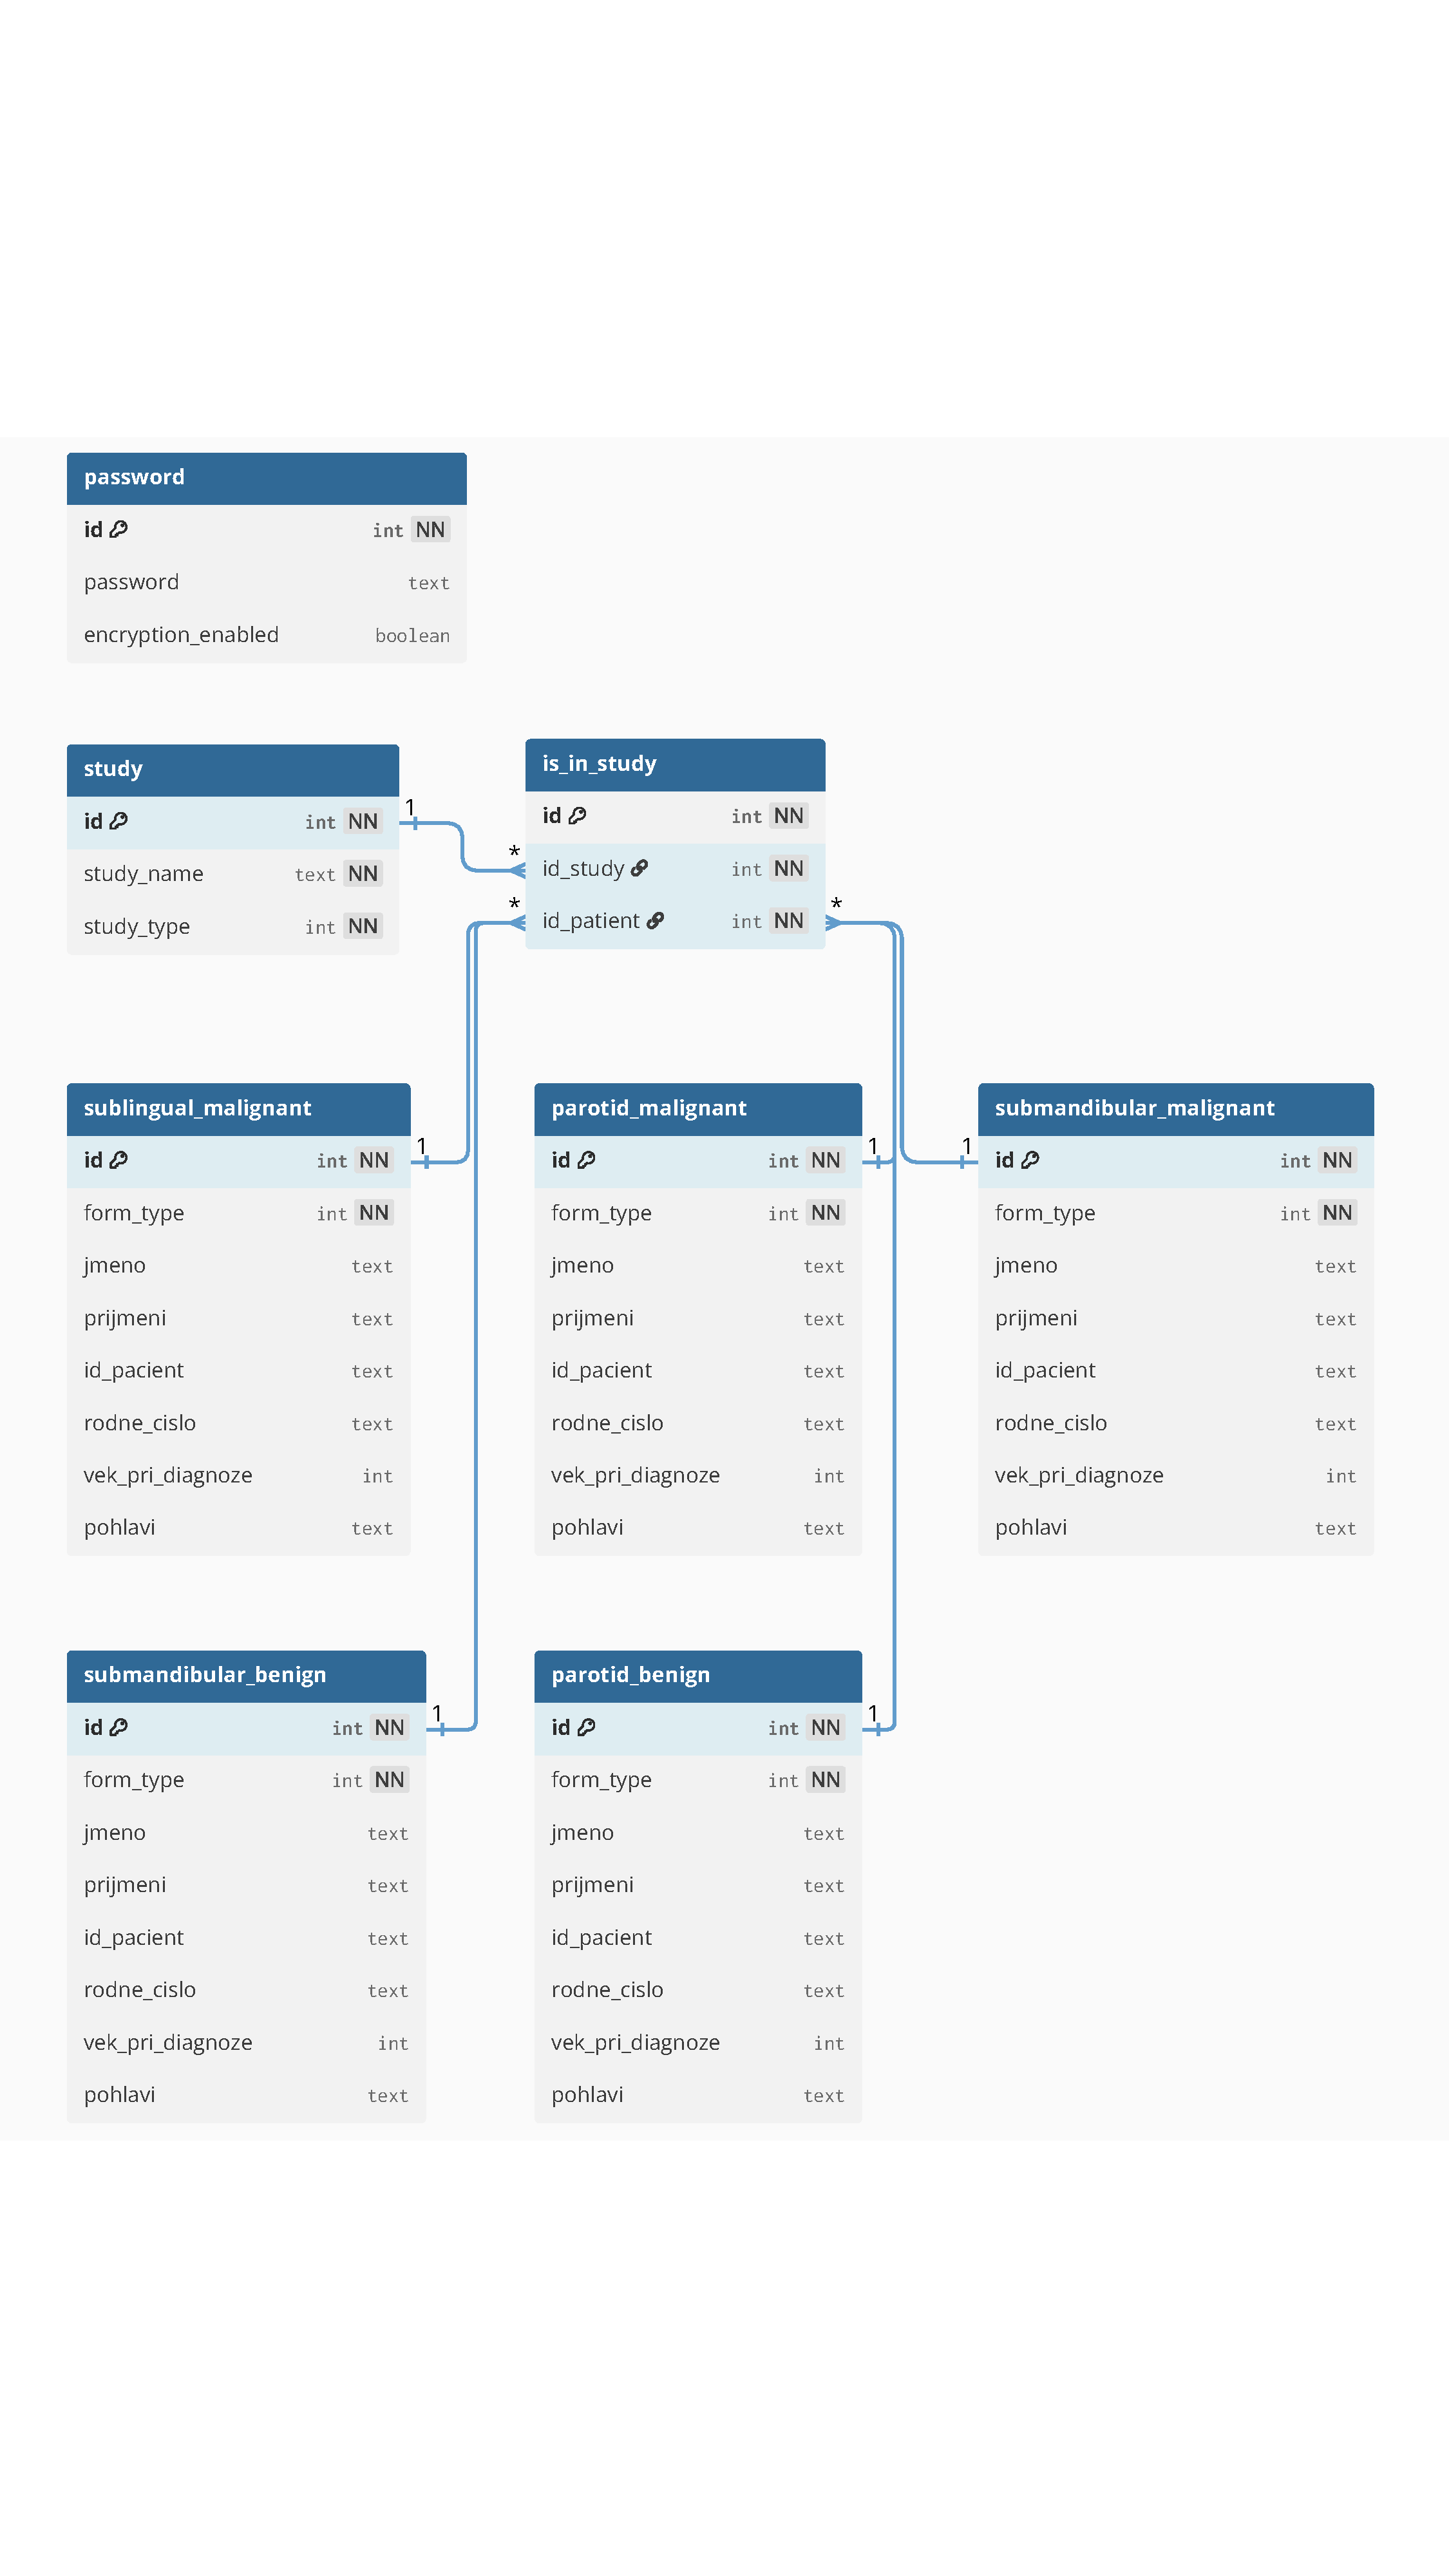
\includegraphics[width=0.95\textwidth]{img/CSGDB_era_simplified.pdf}
    \caption{Zjednodušený ERA diagram databázového schématu SQLite (Entity-Relationship-Attribute).}
    \label{fig:era}
\end{figure}

\subsection{Repozitáře (\texttt{src/backend/repositories/})}
\begin{itemize}
    \item \texttt{patientRepository.ts}: CRUD operace nad pacienty, dynamické skládání SQL pro filtraci a transparentní AES-256-CBC šifrování/dešifrování PII.
    \item \texttt{studyRepository.ts}: Správa výzkumných studií a relací pacientů.
    \item \texttt{tnmRepository.ts}: Dynamická výpočetní logika a pravidla pro TNM stádia.
    \item \texttt{mlRepository.ts}: Persistence metadat ML modelů a uložených predikcí.
    \item \texttt{passwordRepository.ts}: Ověřování hesla a nastavení šifrování.
\end{itemize}

\subsection{Služby a utility backendu}
Uloženy v adresářích \texttt{src/backend/services/} a \texttt{src/backend/utils/}:
\begin{itemize}
    \item \texttt{exportService.ts} / \texttt{importService.ts} / \texttt{importTransformService.ts}: Export/import dat ve formátech JSON a Excel včetně možnosti anonymizace PII.
    \item \texttt{backupService.ts}: Zálohování a obnova SQLite databáze.
    \item \texttt{encryption.ts} / \texttt{patientEncryption.ts}: Kryptografické operace AES-256-CBC s unikátním inicializačním vektorem (IV) pro jméno, příjmení a rodné číslo.
    \item \texttt{mlManager.ts}: Spouštění a řízení běhu binárky Python ML Engine. Podporuje jednorázové spuštění i trvalý \textbf{Sidecar process} (příznak \texttt{--sidecar}), který udržuje proces běžící na pozadí a eliminuje režii opakovaného startu PyInstaller spouštěče.
\end{itemize}

---

\section{Komunikační vrstva --- IPC (\texttt{src/ipc})}

Komunikace mezi klientským Renderer procesem a hlavním Node.js procesem probíhá výhradně asynchronně přes \textbf{Electron IPC}.

\begin{figure}[H]
    \centering
    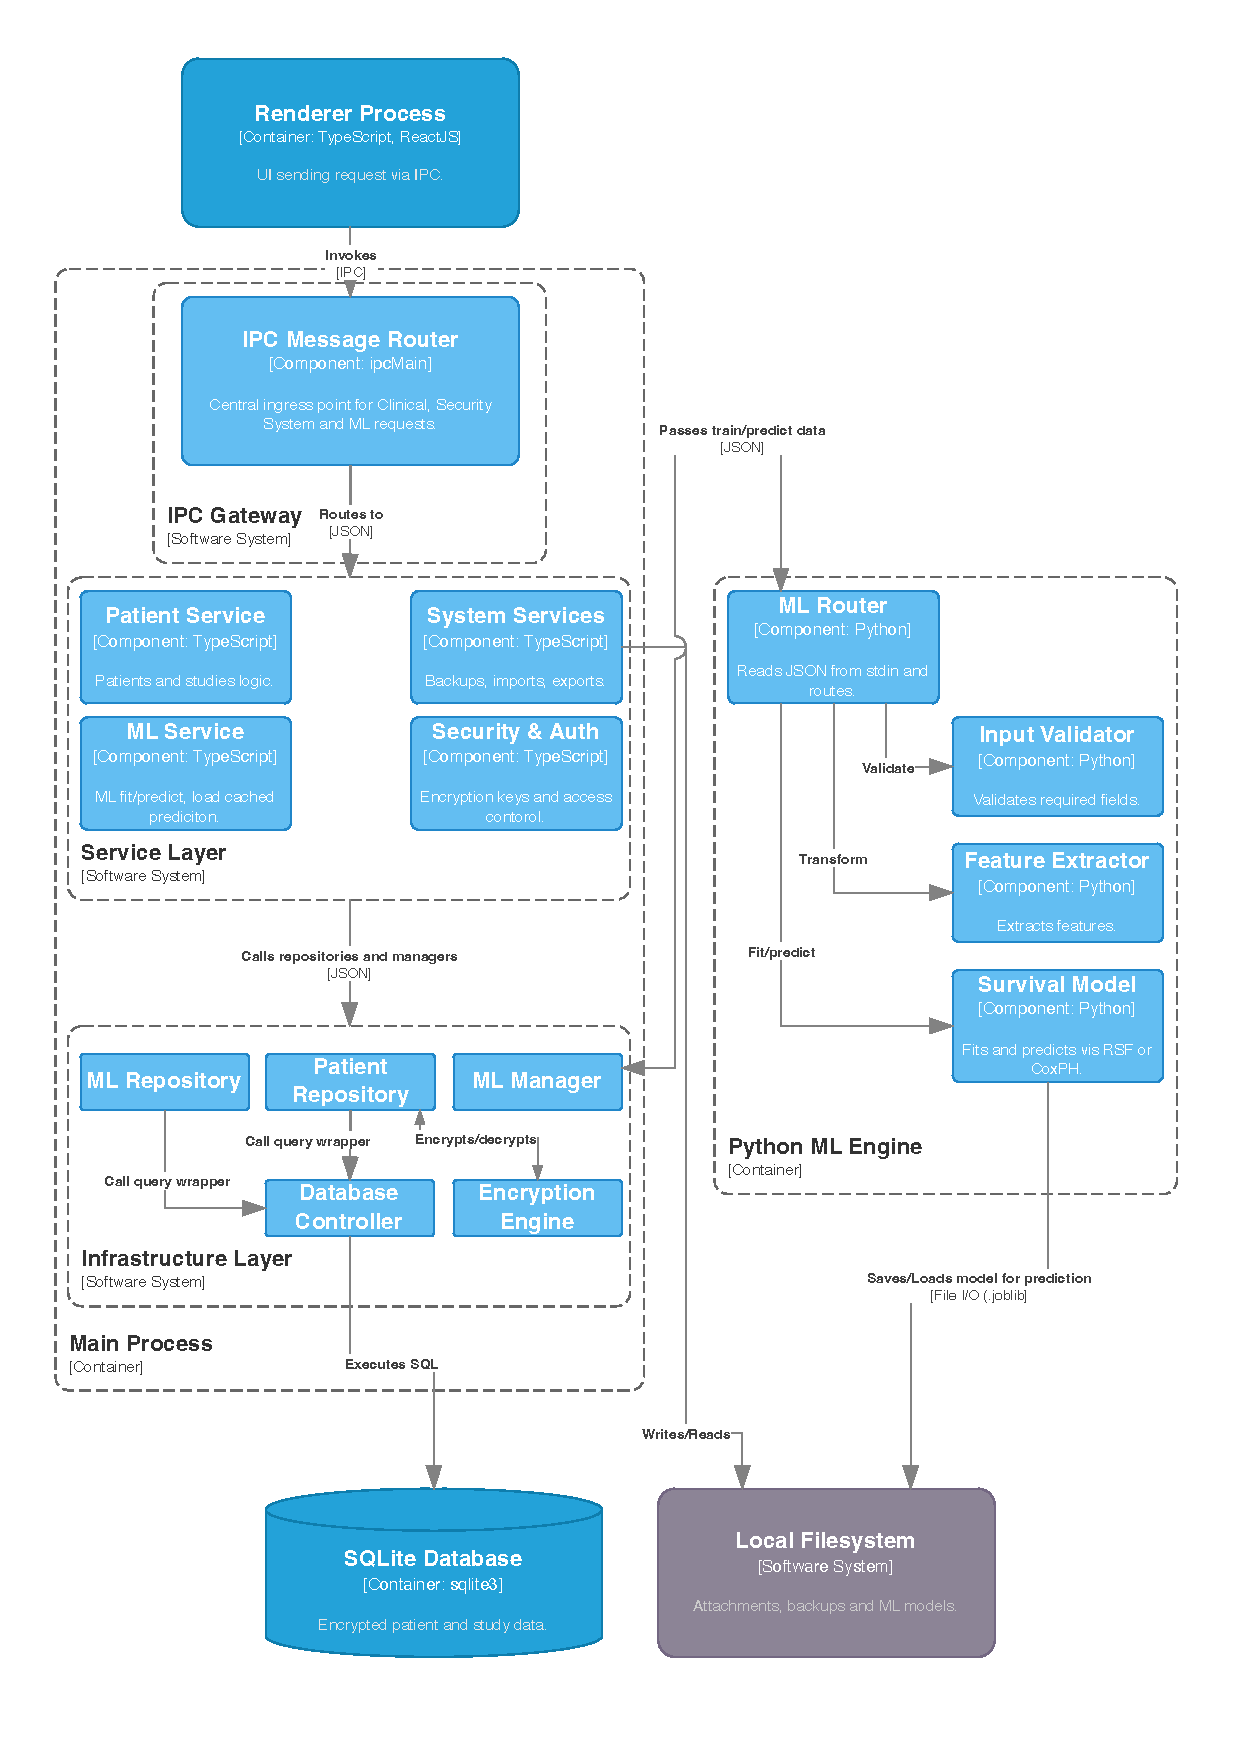
\includegraphics[width=0.95\textwidth]{img/C4-level-3-new.pdf}
    \caption{Diagram komponent systému CSGDB (C4 model --- Level 3).}
    \label{fig:c4-level-3}
\end{figure}

\subsection{Struktura rozhraní IPC}
\begin{itemize}
    \item \texttt{ipcChannels.ts}: Výčtové typy (\texttt{enum}) kanálů:
    \begin{itemize}
        \item API databázové kanály:
        \begin{itemize}
            \item \texttt{ipcAPISaveChannels}, \texttt{ipcAPIInsertChannels}
            \item \texttt{ipcAPIUpdateChannels}, \texttt{ipcAPIDeleteChannels}
            \item \texttt{ipcAPIGetChannels}
        \end{itemize}
        \item Export a import: \texttt{ipcExportChannels}, \texttt{ipcImportChannels}
        \item Souborový systém: \texttt{ipcFSChannels}
        \item Šifrování: \texttt{ipcEncryptionChannels}
        \item Zálohování: \texttt{ipcBackUpChannels}
        \item Strojové učení: \texttt{ipcMLChannels} (\texttt{trainModel}, \texttt{calculateRiskScore}, \texttt{mlProgress}, \texttt{mlCancel})
    \end{itemize}
    \item \textbf{Handlery (\texttt{src/ipc/ipc*Handles.ts}):} Registrace posluchačů v hlavním procesu (\texttt{ipcMain.handle}), které předávají požadavky příslušným backendovým repozitářům.
    \item \textbf{Preload skript (\texttt{src/preload.ts}):} Expozice API do objektu \texttt{window} přes \texttt{contextBridge.exposeInMainWorld} (jmenné prostory \texttt{window.api}, \texttt{window.export}, \texttt{window.import}, \texttt{window.fs}, \texttt{window.encryption}, \texttt{window.backUp}, \texttt{window.ml}).
\end{itemize}

---

\section{Modul strojového učení --- Python ML Engine (\texttt{python-ml-engine})}

Modul \textbf{Python ML Engine} je samostatná jednotka pro analýzu přežití (Survival Analysis) a odhad rizika rekurence či úmrtí pacientů.

\subsection{Technologický stoh modulu}
\begin{itemize}
    \item \textbf{Runtime:} Python 3.8+
    \item \textbf{Závislosti:} \texttt{scikit-survival} (0.22.2), \texttt{scikit-learn} (1.3.2), \texttt{pandas} (2.1.4), \texttt{numpy} (1.24.3).
    \item \textbf{Kompilace:} PyInstaller (binární soubor \texttt{ml\_engine} / \texttt{ml\_engine.exe}).
\end{itemize}

\subsection{Komponenty modulu}
\begin{itemize}
    \item \texttt{ml\_engine.py}: Vstupní bod přijímající JSON přes \texttt{stdin} a vracející JSON na \texttt{stdout}. Operativní režimy: \texttt{train}, \texttt{predict}, \texttt{info} a \texttt{--sidecar}.
    \item \texttt{feature\_extractor.py}: Extrakce a transformace pacientských příznaků:
    \begin{itemize}
        \item \textit{Numerické příznaky:} \texttt{age\_at\_diagnosis}, \texttt{positive\_node\_count}.
        \item \textit{Binární příznaky:} \texttt{lymphatic\_invasion}, \texttt{perineural\_invasion}, \texttt{extranodal\_extension}.
        \item \textit{Kategoriální příznaky:} \texttt{t\_stage} (T1--T4b) a \texttt{grade} (Stage I--IVC) s automatickým fallbackem z patologického na klinické stádium, kódované pomocí One-Hot Encodingu.
        \item \textit{Cílové proměnné (Target):} Čas události v dnech od diagnózy/léčby a status události.
    \end{itemize}
    \item \texttt{survival\_model.py}: Algoritmy \textbf{Random Survival Forest (RSF)} a \textbf{Cox Proportional Hazards (CoxPH)}.
    \item \texttt{validators.py}: Validace JSON schématu vstupních dat.
\end{itemize}

\subsection{Kalkulace skóre rizika}
Skóre rizika představuje doplněk pravděpodobnosti přežití v horizontu 5 let (1825 dní):
\begin{equation}
    \text{Risk Score} = 1.0 - S(t = 1825 \text{ dní})
\end{equation}
kde $S(t)$ je predikovaná funkce přežití. Engine vrací odhady přežití pro 1 rok, 3 roky a 5 let a pořadí významnosti příznaků (Feature Importance).

---

\section{Sestavení a testování}

\subsection{Build Pipeline}
\begin{itemize}
    \item \textbf{Electron Forge \& Webpack:}
    \begin{itemize}
        \item \texttt{webpack.main.config.ts} (main process)
        \item \texttt{webpack.renderer.config.ts} (renderer UI)
    \end{itemize}
    \item \textbf{Extra Resources (\texttt{forge.config.ts}):} Příbal binárního souboru \texttt{ml\_engine} a adresáře předtrénovaných modelů \texttt{pretrained-models/}.
\end{itemize}

\subsection{Testovací sady}
\begin{itemize}
    \item \textbf{Frontend \& IPC:} \textbf{Jest} + \textbf{React Testing Library} (\texttt{npm test}).
    \item \textbf{Python ML Engine:} testovací sada psaná v \textbf{pytest}:
    \begin{itemize}
        \item Jednotkové testy: \texttt{test\_feature\_extractor.py}, \texttt{test\_validators.py}
        \item Integrační testy rozhraní: \texttt{test\_ml\_engine.py}
        \item Verifikační testy: \texttt{sanity\_check.py}
    \end{itemize}
\end{itemize}

\end{document}
